\documentclass[journal]{IEEEtran}
\usepackage[T1]{fontenc}
\usepackage{graphicx}
\usepackage{booktabs}
\usepackage{xcolor}
\usepackage{tikz}
\usetikzlibrary{positioning,calc,arrows.meta,shapes.symbols,shapes.geometric,decorations.pathreplacing}
\usepackage[hidelinks]{hyperref}
\usepackage{cite}

\begin{document}

\title{VeriLoop: Verifiable Digital Service Loops for IoT-Enabled Remote Patient Monitoring}

\author{%
First~Author,
Second~Author,
and~Third~Author%
\thanks{Author affiliations, e-mail addresses and funding acknowledgements to be completed by the authors.}%
}

\maketitle

\begin{abstract}
Remote patient monitoring has made it cheap to collect vital signs at home, but most deployments still stop at an alert:
nobody checks whether the data behind the alert were trustworthy, whether the action that followed actually helped, or
what the system should learn from the outcome. This article argues that connected healthcare needs \emph{verifiable
digital service loops} in which sensing, interpretation, decision, execution and validation form one closed and
auditable cycle. We present VeriLoop, an edge--fog--cloud architecture that (i) diagnoses sensor faults and confirms
suspicious data with the patient before involving clinicians, (ii) maps risk to a tiered service contract bounded by
National Early Warning Score~2 (NEWS2) red-flag guardrails, (iii) verifies the physiological outcome of every clinical
action and escalates when recovery is not observed, (iv) adapts per-patient operating rules only within clinically
approved bounds, and (v) records every loop iteration in a hash-chained provenance ledger anchored in the cloud. In a
reproducible simulation of 150 virtual patients monitored at home for one week under five random seeds (750 patient-weeks), with injected sensor faults and
connectivity outages, VeriLoop let 5.7\% of deterioration episodes reach a critical state, compared with 18.6\% for
continuous NEWS2 monitoring and 11.7\% for an open-loop machine-learning monitor. It also cut false alarms by 38\% and
60\% respectively, and used 59\% less uplink bandwidth than continuous streaming. Removing outcome verification alone
nearly doubled the adverse-event rate. We release the simulator and code, and close with the governance and
regulatory questions that adaptive, closed-loop health services raise.
\end{abstract}

\section*{Introduction}

Internet of Things (IoT) technology has made continuous measurement of heart rate, respiratory rate, oxygen saturation,
blood pressure and temperature possible outside the hospital, and remote patient monitoring (RPM) programmes for chronic
obstructive pulmonary disease (COPD), heart failure and post-discharge care are now common~\cite{islam2015,farahani2018}.
Yet the typical RPM deployment is still device-centric. Data flow from a wearable through a gateway to a cloud
dashboard, a threshold or early-warning score raises an alert, and the loop ends there. Three questions are left
unanswered. Was the alert caused by the patient or by the sensor? Did the clinical action that followed actually work?
And what should the system change, for this patient, as a result? Without answers, RPM services are hard to trust,
generate alarm fatigue~\cite{sendelbach2013}, and cannot produce the evidence that payers and regulators increasingly
expect.

The call for this special issue frames the alternative as a \emph{digital service loop}: a continuous cycle of sensing,
interpretation, decision, execution and validation in which the outcomes of execution feed back into the operational
rules. The idea is related to the MAPE-K loop of autonomic computing~\cite{kephart2003}, but healthcare adds
requirements that generic autonomic loops do not address: actions are carried out by people, not actuators; the cost of
a wrong action is clinical harm; adaptation must stay within limits a clinician can sign off; and every step must be
auditable after the fact.

This article makes four contributions.
\begin{itemize}
\item We define a \emph{verifiable} service loop for home RPM, in which the validation stage has three explicit jobs:
confirming the data, verifying the outcome of each action, and adapting per-patient rules within bounds.
\item We present VeriLoop, an edge--fog--cloud realisation with a tiered service contract, NEWS2
guardrails~\cite{rcp2017}, a fault-aware edge pipeline, a hash-chained provenance ledger and a mapping to HL7
FHIR~\cite{fhir}.
\item We build an open, reproducible closed-loop simulator in which patients deteriorate and respond to treatment,
sensors fail, home connectivity drops out, and patients and clinicians respond to requests with realistic delays.
\item We compare VeriLoop with three common monitoring designs and ablate each loop stage, reporting safety, alarm
burden, energy, bandwidth, latency and audit overhead.
\end{itemize}

\section*{From Monitoring Pipelines to Service Loops}

\subsection*{What Current RPM Systems Do}

IoT health architectures have converged on a layered pattern: body-worn sensors, a smart gateway at the
edge, and cloud analytics~\cite{hassanalieragh2015,rahmani2018}. Moving computation to the edge reduces bandwidth and
latency and keeps working when the backhaul fails~\cite{shi2016}. On the analytics side, aggregate early-warning
scores such as NEWS2 remain the clinical reference: each vital sign is scored 0--3, and an aggregate of 5 or more, or
any single score of 3, triggers urgent review~\cite{rcp2017,smith2013}. Machine-learning models increasingly sit
beside or on top of such scores~\cite{rajkomar2019}.

\subsection*{What Is Missing}

Seen as a loop, these pipelines are open in three places.

\textbf{The data are not validated.} Wearable signals contain motion artefacts, dropouts, frozen values and slowly
drifting probes. Signal-quality indices exist~\cite{orphanidou2015}, but they are usually used to discard samples rather
than to close a loop with the patient (``please re-measure'') or the device (``please re-seat the probe'').

\textbf{The outcome of an action is not verified.} Once an alert has been acknowledged, most systems apply a fixed
cooldown to limit alarm fatigue. If the intervention fails, the system notices only when the cooldown expires and the
patient is, by then, sicker.

\textbf{Operating rules do not learn, or learn without limits.} Static thresholds generate repeated false alarms for
patients whose normal physiology sits outside population norms, while unconstrained adaptive models raise safety and
regulatory concerns about software that changes after approval~\cite{fda2021}.

Finally, few systems can reconstruct \emph{why} a given action was or was not taken. Tamper-evident logs based on
hash chaining~\cite{haber1991} and blockchain-based health-record management~\cite{azaria2016} show that auditability is
technically feasible, but it is rarely built into the monitoring loop itself.

\section*{The VeriLoop Architecture}

Fig.~\ref{fig:arch} shows VeriLoop from two angles. Panel (a) is the deployment: a wearable and a spot-check kit in
the patient's home, an edge gateway (a smartphone or hub) that runs the loop, a care team that acts as the fog tier,
and a cloud that holds the electronic health record and the ledger anchors. Panel (b) is the loop itself. Each
iteration runs once per sample and passes through five stages, and the validation stage feeds back into the earlier
ones.

\begin{figure*}[t]
\centering
\resizebox{\textwidth}{!}{% Fig. 1: VeriLoop overview — (a) deployment view, (b) the verifiable service loop.
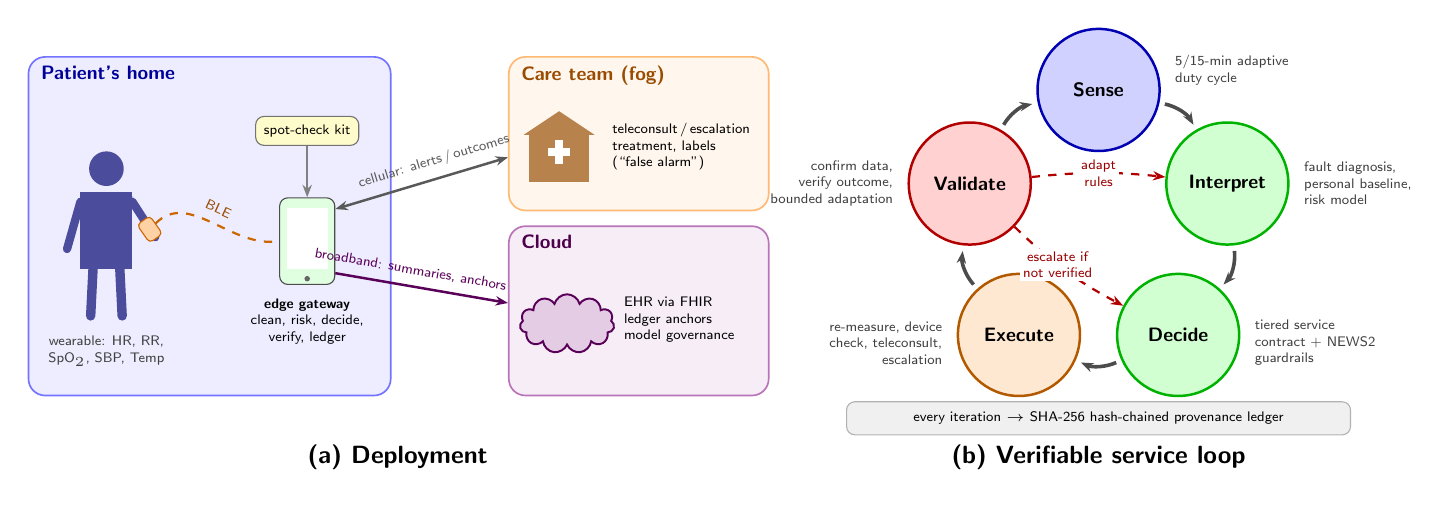
\begin{tikzpicture}[
  font=\sffamily\scriptsize,
  >={Stealth[length=4.5pt]},
  zone/.style={rounded corners=6pt, draw=#1!55, fill=#1!7, line width=0.6pt},
  ztitle/.style={font=\sffamily\scriptsize\bfseries, text=#1!60!black},
  box/.style={rounded corners=3pt, draw=black!55, fill=white, align=center, inner sep=3pt},
  link/.style={->, line width=0.9pt, black!65},
  stage/.style={circle, draw=#1!70!black, fill=#1!18, line width=0.9pt, minimum size=1.55cm, align=center,
                inner sep=0pt, font=\sffamily\scriptsize},
  fb/.style={->, thick, red!70!black, dashed},
  fbl/.style={font=\sffamily\tiny, text=red!60!black, fill=white, inner sep=1pt, align=center},
]
% ====================================================================== (a)
\begin{scope}
\node[zone=blue, minimum width=4.6cm, minimum height=4.3cm, anchor=north west] (home) at (0,0) {};
\node[ztitle=blue, anchor=north west] at (home.north west) {\,Patient's home};
% person
\begin{scope}[shift={(1.0,-2.15)}]
  \fill[blue!45!black!70] (0,0.72) circle (0.22);
  \fill[blue!45!black!70] (-0.33,-0.55) rectangle (0.33,0.42);
  \fill[blue!45!black!70, rounded corners=2pt] (-0.33,0.42) -- (0.33,0.42) -- (0.33,0.3) -- (-0.33,0.3) -- cycle;
  \draw[blue!45!black!70, line width=3pt, line cap=round] (0.33,0.3) -- (0.62,-0.15);
  \draw[blue!45!black!70, line width=3pt, line cap=round] (-0.33,0.3) -- (-0.5,-0.3);
  \draw[blue!45!black!70, line width=3.4pt, line cap=round] (-0.17,-0.55) -- (-0.2,-1.15);
  \draw[blue!45!black!70, line width=3.4pt, line cap=round] (0.17,-0.55) -- (0.2,-1.15);
  % wearable
  \node[draw=orange!80!black, fill=orange!35, rounded corners=1.5pt, minimum width=0.28cm, minimum height=0.2cm,
        inner sep=0pt, rotate=-55] (watch) at (0.55,-0.05) {};
\end{scope}
\node[font=\sffamily\tiny, align=center, text=black!75] at (1.0,-3.75) {wearable: HR, RR,\\SpO$_2$, SBP, Temp};
% gateway (phone)
\node[draw=black!70, fill=green!12, rounded corners=3pt, minimum width=0.7cm, minimum height=1.1cm] (gw) at (3.55,-2.35) {};
\fill[white] ($(gw.center)+(-0.26,-0.36)$) rectangle ($(gw.center)+(0.26,0.42)$);
\fill[black!60] ($(gw.south)+(0,0.08)$) circle (0.035);
\node[font=\sffamily\tiny, align=center, anchor=north] at ($(gw.south)+(0,-0.05)$) {\textbf{edge gateway}\\clean, risk, decide,\\verify, ledger};
\draw[dashed, orange!80!black, thick] (watch) .. controls +(0.5,0.5) and +(-0.6,-0.1) .. node[above, sloped, font=\sffamily\tiny, text=orange!60!black]{BLE} (gw.west);
% spot-check device
\node[box, font=\sffamily\tiny, fill=yellow!20] (spot) at (3.55,-0.95) {spot-check kit};
\end{scope}

% care team (fog)
\begin{scope}[shift={(6.1,0)}]
\node[zone=orange, minimum width=3.3cm, minimum height=1.95cm, anchor=north west] (care) at (0,0) {};
\node[ztitle=orange, anchor=north west] at (care.north west) {\,Care team (fog)};
% clinic icon
\begin{scope}[shift={(0.65,-1.25)}]
  \fill[orange!60!black!70] (-0.38,-0.35) rectangle (0.38,0.25);
  \fill[orange!60!black!70] (-0.45,0.25) -- (0,0.55) -- (0.45,0.25) -- cycle;
  \fill[white] (-0.05,-0.12) rectangle (0.05,0.18);
  \fill[white] (-0.14,-0.02) rectangle (0.14,0.08);
\end{scope}
\node[font=\sffamily\tiny, align=left, anchor=west] at (1.2,-1.15) {teleconsult\,/\,escalation\\treatment, labels\\(``false alarm'')};

\node[zone=violet, minimum width=3.3cm, minimum height=2.15cm, anchor=north west] (cloud) at (0,-2.15) {};
\node[ztitle=violet, anchor=north west] at (cloud.north west) {\,Cloud};
\node[cloud, cloud puffs=11, draw=violet!70!black, fill=violet!20, minimum width=1.2cm, minimum height=0.75cm,
      line width=0.7pt] at (0.75,-3.4) {};
\node[font=\sffamily\tiny, align=left, anchor=west] at (1.35,-3.35) {EHR via FHIR\\ledger anchors\\model governance};
\end{scope}

\draw[link, <->] ($(gw.north east)+(0,-0.15)$) -- node[above, sloped, font=\sffamily\tiny, pos=0.6]{cellular: alerts\,/\,outcomes} ($(care.west)+(0,-0.3)$);
\draw[link, violet!70!black] ($(gw.south east)+(0,0.15)$) -- node[above, sloped, font=\sffamily\tiny, pos=0.42]{broadband: summaries, anchors} ($(cloud.west)+(0,0.1)$);
\draw[link, black!50] (spot.south) -- (gw.north);
\node[font=\sffamily\bfseries\small] at (4.7,-5.1) {(a) Deployment};

% ====================================================================== (b)
\begin{scope}[shift={(13.6,-2.15)}]
\def\R{1.72}
\node[stage=blue]   (s1) at (90:\R)   {\textbf{Sense}};
\node[stage=green]  (s2) at (18:\R)   {\textbf{Interpret}};
\node[stage=green]  (s3) at (-54:\R)  {\textbf{Decide}};
\node[stage=orange] (s4) at (-126:\R) {\textbf{Execute}};
\node[stage=red]    (s5) at (162:\R)  {\textbf{Validate}};
\foreach \a/\b in {s1/s2, s2/s3, s3/s4, s4/s5, s5/s1}
  \draw[->, line width=1.3pt, black!70, shorten >=2pt, shorten <=2pt] (\a) to[bend left=24] (\b);
% feedback chords from Validate
\draw[fb] (s5) to[bend right=8] node[fbl, pos=0.42]{escalate if\\not verified} (s3);
\draw[fb] (s5) to[bend left=6] node[fbl, pos=0.5]{adapt\\rules} (s2);
% stage annotations outside the wheel
\node[font=\sffamily\tiny, align=left, anchor=west, text=black!75] at ($(s1)+(0.85,0.25)$) {5/15-min adaptive\\duty cycle};
\node[font=\sffamily\tiny, align=left, anchor=west, text=black!75] at ($(s2)+(0.85,0)$) {fault diagnosis,\\personal baseline,\\risk model};
\node[font=\sffamily\tiny, align=left, anchor=west, text=black!75] at ($(s3)+(0.85,-0.1)$) {tiered service\\contract + NEWS2\\guardrails};
\node[font=\sffamily\tiny, align=right, anchor=east, text=black!75] at ($(s4)+(-0.85,-0.1)$) {re-measure, device\\check, teleconsult,\\escalation};
\node[font=\sffamily\tiny, align=right, anchor=east, text=black!75] at ($(s5)+(-0.85,0)$) {confirm data,\\verify outcome,\\bounded adaptation};
% ledger bar
\node[draw=gray!60, fill=gray!12, rounded corners=3pt, minimum width=6.4cm, minimum height=0.42cm,
      font=\sffamily\tiny, align=center] at (0,-2.45) {every iteration $\rightarrow$ SHA-256 hash-chained provenance ledger};
\node[font=\sffamily\bfseries\small] at (0,-2.95) {(b) Verifiable service loop};
\end{scope}
\end{tikzpicture}
}
\caption{VeriLoop at a glance. (a) Deployment: the home edge gateway runs the loop, alerts travel over a cellular
fallback, and only summaries and hourly ledger anchors go over the home broadband. (b) The verifiable service loop:
validation feeds back into decision (escalate when recovery is not verified) and interpretation (bounded adaptation),
and every iteration is written to a hash-chained provenance ledger.}
\label{fig:arch}
\end{figure*}

\subsection*{Sense}

The wearable reports the five NEWS2 vital signs that can be measured without a clinician. To save energy, it runs a
two-rate duty cycle: one sample every 15 minutes while the patient is stable, and one every 5 minutes as soon as the
edge sees any sign of risk.

\subsection*{Interpret}

The edge gateway cleans each sample before it is used. Values outside physiological ranges are rejected. A jump larger
than a channel-specific limit is held back until the next sample confirms it, so single-sample motion spikes never reach
the decision stage, while a genuine change is accepted five minutes later. A channel that repeats exactly the same value
for longer than is physiologically plausible is marked as frozen. Finally, an isolated deviation of oxygen saturation or
blood pressure that is not corroborated by any other vital sign is marked as \emph{suspect}, because probe displacement
and cuff errors are far more common than an isolated real change.

The cleaned values are compared with a personal baseline learned over the first 24 hours of monitoring. A
logistic-regression risk model at the fog tier turns 16 personalised features (current deviation, one-hour mean
deviation and 30-minute trend of each vital sign, plus the NEWS2 aggregate) into a deterioration risk between 0 and 1.
We deliberately chose a simple, inspectable model: each coefficient can be reviewed by a clinician, which matters more
for a regulated service than a small gain in discrimination.

\subsection*{Decide: A Tiered Service Contract}

The decision stage maps risk to four tiers, each tied to a service-level commitment:
\begin{itemize}
\item \emph{Tier 0, routine}: low-rate sensing and a summary upload every 30 minutes.
\item \emph{Tier 1, patient/device request}: ask the patient to rest and re-measure with a spot-check device, or to
re-seat a sensor; answered within minutes, with no clinician involved.
\item \emph{Tier 2, teleconsultation}: triggered when the personal risk exceeds the patient's threshold, or NEWS2
reaches the amber level (aggregate 5, or a single parameter scoring 3), for two consecutive samples.
\item \emph{Tier 3, emergency escalation}: NEWS2 aggregate 7 or more, or very high risk.
\end{itemize}
Two design rules keep this safe. First, every Tier~2 trigger and every Tier~3 trigger that rests on a single vital
sign is confirmed by a Tier~1 re-measurement before a clinician is called, and a request that goes unanswered escalates
anyway. Second, the NEWS2 red-flag rules are \emph{guardrails}: the adaptation described below can never relax them.

\subsection*{Execute}

Actions are requests to people or devices, so execution is asynchronous. VeriLoop tracks each one as an open service
request with a deadline. The edge sends Tier~2 and Tier~3 requests over the cellular network when the home broadband is
down, so a connectivity outage delays only the routine upload, not the alert.

\subsection*{Validate}

Validation does three jobs.
\begin{itemize}
\item \emph{Confirm the data.} If a re-measurement contradicts the wearable, the trigger is cancelled, the channel is
flagged and a device check is requested. This closes the loop back to sensing.
\item \emph{Verify the outcome.} When a clinician reports that treatment has started, VeriLoop schedules a check 90
minutes later. If neither the risk nor the NEWS2 aggregate has fallen, it escalates to Tier~3 immediately instead of
waiting for an alarm cooldown to expire.
\item \emph{Adapt within bounds.} When a clinician labels an alert as a false alarm, VeriLoop raises that patient's
risk threshold by 0.05 (to at most 0.85), may raise the NEWS2 amber threshold from 5 to 6 (never higher), and nudges
the personal baseline toward recent stable values. The red-flag guardrails are never changed. These bounds are the
kind of pre-specified change envelope that regulators now ask manufacturers of adaptive software to declare in
advance~\cite{fda2021}.
\end{itemize}

Fig.~\ref{fig:lifecycle} follows one service request through the loop, from the first abnormal sample to verified
recovery.

\begin{figure*}[t]
\centering
\resizebox{\textwidth}{!}{% Fig. 2: lifecycle of one verified service request (swimlane / sequence view)
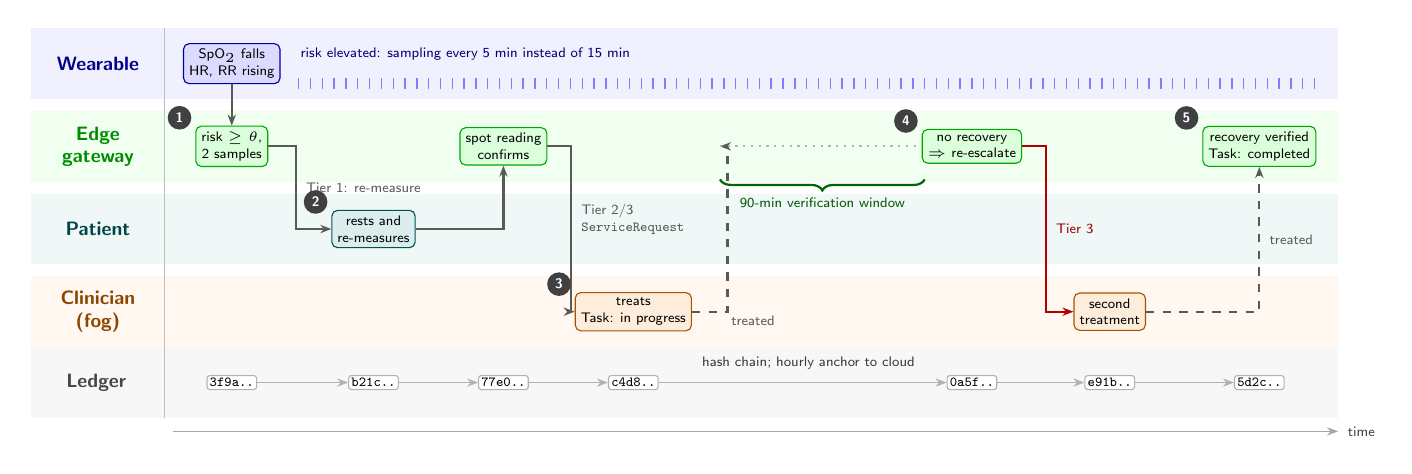
\begin{tikzpicture}[
  font=\sffamily\scriptsize,
  >={Stealth[length=4pt]},
  lane/.style={fill=#1!6, draw=none},
  lname/.style={font=\sffamily\scriptsize\bfseries, text=#1!55!black, align=center, text width=1.55cm},
  ev/.style={rounded corners=2pt, draw=#1!65!black, fill=#1!14, align=center, inner sep=2pt, font=\sffamily\tiny},
  msg/.style={->, thick, black!65},
  bad/.style={->, thick, red!70!black},
  num/.style={circle, fill=black!75, text=white, font=\sffamily\tiny\bfseries, inner sep=0pt, minimum size=0.3cm},
  hash/.style={draw=gray!60, fill=white, font=\ttfamily\tiny, inner sep=1pt, rounded corners=1pt},
]
\def\W{16.6}
% lanes (y positions)
\def\yW{0} \def\yE{-1.05} \def\yP{-2.1} \def\yC{-3.15} \def\yL{-4.05}
\foreach \y/\c/\n in {\yW/blue/Wearable, \yE/green/Edge gateway, \yP/teal/Patient, \yC/orange/Clinician (fog), \yL/gray/Ledger\,/\,cloud}{
  \fill[lane=\c] (0,\y-0.45) rectangle (\W,\y+0.45);
  \node[lname=\c] at (0.85,\y) {\n};
}
\draw[gray!50] (1.7,0.45) -- (1.7,\yL-0.45);
% time axis
\draw[->, gray!70] (1.8,\yL-0.62) -- (\W,\yL-0.62) node[right, font=\sffamily\tiny, text=gray!50!black]{time};

% 1: anomaly
\node[ev=blue] (a1) at (2.55,\yW) {SpO$_2$ falls\\HR, RR rising};
\node[ev=green] (b1) at (2.55,\yE) {risk $\geq\theta$,\\2 samples};
\draw[msg] (a1) -- (b1);
\node[num] at ($(b1.north west)+(-0.2,0.1)$) {1};
% 2: confirm with patient
\node[ev=teal] (p1) at (4.35,\yP) {rests and\\re-measures};
\draw[msg] (b1.east) -- ++(0.35,0) |- node[pos=0.25, right, font=\sffamily\tiny]{Tier 1: re-measure} (p1.west);
\node[ev=green] (b2) at (6.0,\yE) {spot reading\\confirms};
\draw[msg] (p1.east) -| (b2.south);
\node[num] at ($(p1.north west)+(-0.2,0.1)$) {2};
% 3: escalate
\node[ev=orange] (c1) at (7.65,\yC) {treats\\Task: in progress};
\draw[msg] (b2.east) -- ++(0.3,0) |- node[pos=0.22, right, font=\sffamily\tiny, align=left]{Tier 2/3\\\texttt{ServiceRequest}} (c1.west);
\node[num] at ($(c1.north west)+(-0.2,0.1)$) {3};
% 4: verification window
\draw[decorate, decoration={brace, amplitude=4pt, mirror}, thick, green!40!black] (8.75,\yE-0.42) -- node[below=3pt, font=\sffamily\tiny, text=green!35!black]{90-min verification window} (11.35,\yE-0.42);
\node[ev=green] (b3) at (11.95,\yE) {no recovery\\$\Rightarrow$ re-escalate};
\draw[msg, dashed] (c1.east) -- ++(0.45,0) node[below right, font=\sffamily\tiny, inner sep=1pt]{treated} |- (8.75,\yE);
\draw[gray!60, dotted, thick] (8.75,\yE) -- (b3.west);
\node[num] at ($(b3.north west)+(-0.2,0.1)$) {4};
\node[ev=orange] (c2) at (13.7,\yC) {second\\treatment};
\draw[bad] (b3.east) -- ++(0.3,0) |- node[pos=0.25, right, font=\sffamily\tiny, text=red!60!black]{Tier 3} (c2.west);
\node[ev=green] (b4) at (15.6,\yE) {recovery verified\\Task: completed};
\draw[msg, dashed] (c2.east) -| node[pos=0.75, right, font=\sffamily\tiny]{treated} (b4.south);
\node[num] at ($(b4.north west)+(-0.2,0.1)$) {5};

% sampling ticks on the wearable lane
\foreach \x in {3.4,3.55,...,16.4} \draw[blue!50, line width=0.5pt] (\x,\yW-0.32) -- (\x,\yW-0.18);
\node[font=\sffamily\tiny, text=blue!45!black, anchor=west] at (3.3,\yW+0.12) {risk elevated: sampling every 5 min instead of 15 min};
% ledger: hashes under every step
\foreach \x/\h [count=\i] in {2.55/{3f9a..}, 4.35/{b21c..}, 6.0/{77e0..}, 7.65/{c4d8..}, 11.95/{0a5f..}, 13.7/{e91b..}, 15.6/{5d2c..}}{
  \node[hash] (h\i) at (\x,\yL) {\h};
}
\foreach \a [evaluate=\a as \b using int(\a+1)] in {1,...,6}
  \draw[->, gray!60] (h\a) -- (h\b);
\node[font=\sffamily\tiny, text=gray!45!black, anchor=west] at (8.4,\yL+0.25) {hash chain; hourly anchor to cloud};
\end{tikzpicture}
}
\caption{Lifecycle of one verified service request. (1) The edge detects rising risk and raises the sampling rate.
(2) Before calling a clinician it asks the patient to re-measure. (3) The confirmed reading becomes a Tier~2/3
\texttt{ServiceRequest}, and the clinician starts treatment. (4) Ninety minutes later no recovery is visible, so the
edge escalates again instead of waiting for an alarm cooldown. (5) Recovery after the second treatment is verified and
the \texttt{Task} is closed. Each step adds a link to the hash chain.}
\label{fig:lifecycle}
\end{figure*}

\subsection*{Provenance and Interoperability}

Every loop iteration (observation digest, quality flags, risk, tier, threshold and any action or feedback) is
serialised and appended to a SHA-256 hash chain at the edge~\cite{haber1991}. Every hour the head of the chain is sent
to the cloud as an anchor. Anyone holding the anchors can later prove that the edge log was not edited, reordered or cut
short. For exchange with electronic health records, observations map to FHIR \texttt{Observation} resources, requests
to \texttt{ServiceRequest} and \texttt{Task}, and each decision carries a \texttt{Provenance} resource whose signature
field holds the ledger hash~\cite{fhir}.

\section*{Evaluation Methodology}

Evaluating a closed loop needs an environment that reacts: an alert must be able to change what the patient's vital
signs do next. Retrospective datasets cannot provide this, so we built a discrete-event simulator. All parameters are in
the released code. We stress that the results below come from simulation and are meant to compare loop designs under
identical, controlled conditions, not to estimate clinical effect sizes. Fig.~\ref{fig:method} summarises the
methodology.

\begin{figure*}[t]
\centering
\resizebox{\textwidth}{!}{% Fig. 3: evaluation methodology (closed-loop simulation pipeline)
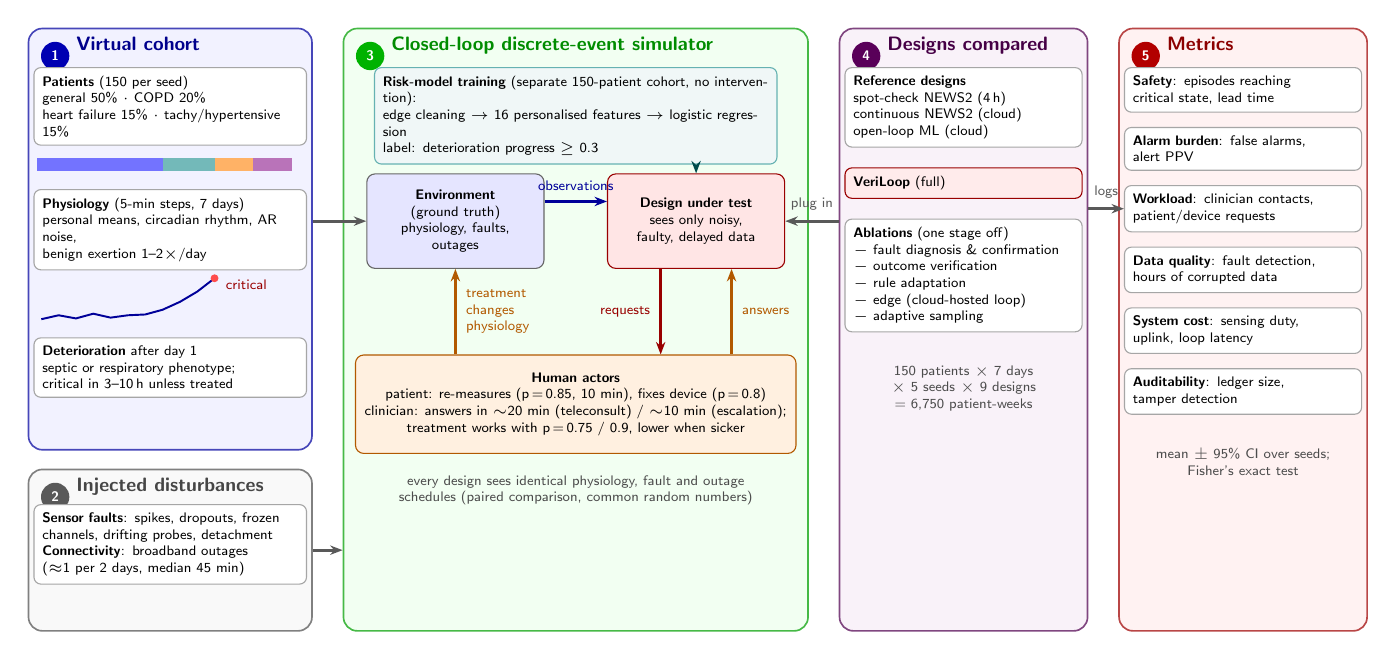
\begin{tikzpicture}[
  font=\sffamily\scriptsize,
  >={Stealth[length=4.5pt]},
  panel/.style={rounded corners=5pt, draw=#1!45!gray, fill=#1!5, line width=0.6pt},
  ptitle/.style={font=\sffamily\scriptsize\bfseries, text=#1!55!black, anchor=north west},
  item/.style={rounded corners=2.5pt, draw=black!35, fill=white, align=left, text width=#1, inner sep=3pt,
               font=\sffamily\tiny},
  it/.style={rounded corners=2.5pt, draw=black!35, fill=white, align=left, inner sep=3pt, font=\sffamily\tiny},
  arr/.style={->, line width=1.1pt, black!65},
  loop/.style={->, line width=1pt, #1},
  badge/.style={circle, fill=#1!70!black, text=white, font=\sffamily\tiny\bfseries, inner sep=1.2pt, minimum size=0.36cm},
]
% ---------------------------------------------------------------- column 1
\node[panel=blue, minimum width=3.6cm, minimum height=5.35cm, anchor=north west] (c1) at (0,0) {};
\node[ptitle=blue] at (c1.north west) {\,\tikz[baseline=-0.6ex]\node[badge=blue]{1};\ Virtual cohort};
\node[it, text width=3.25cm, anchor=north] (g) at ($(c1.north)+(0,-0.5)$)
  {\textbf{Patients} (150 per seed)\\general 50\% $\cdot$ COPD 20\%\\heart failure 15\% $\cdot$ tachy/hypertensive 15\%};
% little population bar
\begin{scope}[shift={($(g.south west)+(0.05,-0.32)$)}]
  \fill[blue!55] (0,0) rectangle (1.6,0.16);
  \fill[teal!55] (1.6,0) rectangle (2.25,0.16);
  \fill[orange!60] (2.25,0) rectangle (2.74,0.16);
  \fill[violet!55] (2.74,0) rectangle (3.23,0.16);
\end{scope}
\node[it, text width=3.25cm, anchor=north] (ph) at ($(g.south)+(0,-0.55)$)
  {\textbf{Physiology} (5-min steps, 7 days)\\personal means, circadian rhythm, AR noise,\\benign exertion 1--2$\times$/day};
% tiny vital-sign sparkline
\draw[blue!60!black, line width=0.7pt] ($(ph.south west)+(0.1,-0.62)$)
   -- ++(0.22,0.05) -- ++(0.22,-0.04) -- ++(0.22,0.06) -- ++(0.22,-0.05) -- ++(0.22,0.03) -- ++(0.22,0.01)
   -- ++(0.22,0.06) -- ++(0.22,0.1) -- ++(0.22,0.13) -- ++(0.22,0.17) coordinate (spk);
\fill[red!70] (spk) circle (0.05);
\node[font=\sffamily\tiny, text=red!60!black, anchor=west] at ($(spk)+(0.02,-0.08)$) {critical};
\node[it, text width=3.25cm, anchor=north] (ep) at ($(ph.south)+(0,-0.85)$)
  {\textbf{Deterioration} after day 1\\septic or respiratory phenotype;\\critical in 3--10\,h unless treated};

% ---------------------------------------------------------------- column 1b: disturbances
\node[panel=gray, minimum width=3.6cm, minimum height=2.05cm, anchor=north west] (c1b) at (0,-5.6) {};
\node[ptitle=gray] at (c1b.north west) {\,\tikz[baseline=-0.6ex]\node[badge=gray]{2};\ Injected disturbances};
\node[it, text width=3.25cm, anchor=north] at ($(c1b.north)+(0,-0.45)$)
  {\textbf{Sensor faults}: spikes, dropouts, frozen\\channels, drifting probes, detachment\\\textbf{Connectivity}: broadband outages\\($\approx$1 per 2 days, median 45 min)};

% ---------------------------------------------------------------- column 2: simulator
\node[panel=green, minimum width=5.9cm, minimum height=7.65cm, anchor=north west] (c2) at (4.0,0) {};
\node[ptitle=green] at (c2.north west) {\,\tikz[baseline=-0.6ex]\node[badge=green]{3};\ Closed-loop discrete-event simulator};
% training box at top
\node[item=4.9cm, draw=teal!60, fill=teal!6, anchor=north] (train) at ($(c2.north)+(0,-0.5)$)
  {\textbf{Risk-model training} (separate 150-patient cohort, no intervention):\\edge cleaning $\rightarrow$ 16 personalised features $\rightarrow$ logistic regression\\label: deterioration progress $\geq$ 0.3};
\node[rounded corners=3pt, draw=black!60, fill=blue!10, minimum width=2.25cm, minimum height=1.2cm, align=center,
      font=\sffamily\tiny, anchor=north west] (env) at ($(c2.north west)+(0.3,-1.85)$)
  {\textbf{Environment}\\(ground truth)\\physiology, faults,\\outages};
\node[rounded corners=3pt, draw=red!60!black, fill=red!10, minimum width=2.25cm, minimum height=1.2cm, align=center,
      font=\sffamily\tiny, anchor=north east] (dut) at ($(c2.north east)+(-0.3,-1.85)$)
  {\textbf{Design under test}\\sees only noisy,\\faulty, delayed data};
\node[rounded corners=3pt, draw=orange!70!black, fill=orange!12, minimum width=5.3cm, minimum height=1.25cm, align=center,
      font=\sffamily\tiny, anchor=north] (hum) at ($(c2.north)+(0,-4.15)$)
  {\textbf{Human actors}\\patient: re-measures (p\,=\,0.85, 10 min), fixes device (p\,=\,0.8)\\clinician: answers in $\sim$20 min (teleconsult) / $\sim$10 min (escalation);\\treatment works with p\,=\,0.75 / 0.9, lower when sicker};
\draw[loop=blue!60!black] ($(env.east)+(0,0.25)$) -- node[above, font=\sffamily\tiny]{observations} ($(dut.west)+(0,0.25)$);
\coordinate (rq1) at ($(dut.south)+(-0.45,0)$);
\coordinate (an1) at ($(dut.south)+(0.45,0)$);
\draw[loop=red!60!black] (rq1) -- node[left, font=\sffamily\tiny]{requests} (rq1 |- hum.north);
\draw[loop=orange!70!black] (an1 |- hum.north) -- node[right, font=\sffamily\tiny]{answers} (an1);
\draw[loop=orange!70!black] (hum.north -| env.south) -- node[right, font=\sffamily\tiny, align=left]{treatment\\changes\\physiology} (env.south);
\draw[arr, teal!60!black] (train.south -| dut.north) -- (dut.north);
\node[font=\sffamily\tiny, align=center, text=black!70, anchor=north] at ($(hum.south)+(0,-0.15)$)
  {every design sees identical physiology, fault and outage\\schedules (paired comparison, common random numbers)};

% ---------------------------------------------------------------- column 3: designs
\node[panel=violet, minimum width=3.15cm, minimum height=7.65cm, anchor=north west] (c3) at (10.3,0) {};
\node[ptitle=violet] at (c3.north west) {\,\tikz[baseline=-0.6ex]\node[badge=violet]{4};\ Designs compared};
\node[it, text width=2.8cm, anchor=north] (ref) at ($(c3.north)+(0,-0.5)$)
  {\textbf{Reference designs}\\spot-check NEWS2 (4\,h)\\continuous NEWS2 (cloud)\\open-loop ML (cloud)};
\node[it, text width=2.8cm, anchor=north, draw=red!60!black, fill=red!8] (vl) at ($(ref.south)+(0,-0.25)$)
  {\textbf{VeriLoop} (full)};
\node[it, text width=2.8cm, anchor=north] (abl) at ($(vl.south)+(0,-0.25)$)
  {\textbf{Ablations} (one stage off)\\$-$ fault diagnosis \& confirmation\\$-$ outcome verification\\$-$ rule adaptation\\$-$ edge (cloud-hosted loop)\\$-$ adaptive sampling};
\node[font=\sffamily\tiny, align=center, text=black!70, anchor=north] at ($(abl.south)+(0,-0.3)$)
  {150 patients $\times$ 7 days\\$\times$ 5 seeds $\times$ 9 designs\\= 6{,}750 patient-weeks};

% ---------------------------------------------------------------- column 4: metrics
\node[panel=red, minimum width=3.15cm, minimum height=7.65cm, anchor=north west] (c4) at (13.85,0) {};
\node[ptitle=red] at (c4.north west) {\,\tikz[baseline=-0.6ex]\node[badge=red]{5};\ Metrics};
\node[it, text width=2.8cm, anchor=north] (m1) at ($(c4.north)+(0,-0.5)$) {\textbf{Safety}: episodes reaching\\critical state, lead time};
\node[it, text width=2.8cm, anchor=north] (m2) at ($(m1.south)+(0,-0.18)$) {\textbf{Alarm burden}: false alarms,\\alert PPV};
\node[it, text width=2.8cm, anchor=north] (m3) at ($(m2.south)+(0,-0.18)$) {\textbf{Workload}: clinician contacts,\\patient/device requests};
\node[it, text width=2.8cm, anchor=north] (m4) at ($(m3.south)+(0,-0.18)$) {\textbf{Data quality}: fault detection,\\hours of corrupted data};
\node[it, text width=2.8cm, anchor=north] (m5) at ($(m4.south)+(0,-0.18)$) {\textbf{System cost}: sensing duty,\\uplink, loop latency};
\node[it, text width=2.8cm, anchor=north] (m6) at ($(m5.south)+(0,-0.18)$) {\textbf{Auditability}: ledger size,\\tamper detection};
\node[font=\sffamily\tiny, align=center, text=black!70, anchor=north] at ($(m6.south)+(0,-0.3)$) {mean $\pm$ 95\% CI over seeds;\\Fisher's exact test};

% ---------------------------------------------------------------- flow arrows between columns
\draw[arr] (c1.east |- env.west) ++(0,0) -- (env.west);
\draw[arr] (c1b.east) -- (c1b.east -| c2.west);
\draw[arr] (c3.west |- dut.east) -- node[above, font=\sffamily\tiny]{plug in} (dut.east);
\draw[arr] (c3.east |- m3.west) -- node[above, font=\sffamily\tiny]{logs} (m3.west);
\end{tikzpicture}
}
\caption{Evaluation methodology. A virtual cohort (1) and injected sensor faults and outages (2) drive a closed-loop
simulator (3) in which the design under test sees only what a real deployment would see, and its requests are answered
by simulated patients and clinicians whose treatments change the physiology. Every design (4) runs on identical
schedules, and the logs are scored on six groups of metrics (5).}
\label{fig:method}
\end{figure*}

\textbf{Virtual cohort.} Each patient is monitored at home for seven days at 5-minute resolution. Patients are drawn
from four sub-groups: general older adults (50\%), COPD (20\%, scored on the NEWS2 SpO$_2$ scale~2), heart failure on
rate control (15\%), and patients with resting tachycardia and hypertension (15\%). Vital signs combine personal means,
circadian rhythm, autocorrelated noise and one to two benign exertion episodes per day. About 40\% of patients develop
one or more deterioration episodes after the first day, with either a septic or a respiratory phenotype. Untreated, an
episode reaches a critical state in 3--10 hours; we count reaching that state as an adverse event.

\textbf{Faults and connectivity.} Each patient's devices suffer motion spikes, dropouts, frozen channels, drifting
SpO$_2$ probes and blood-pressure cuffs, and detached probes, at rates of a few events per day, along with home-broadband
outages averaging one every two days (median 45 minutes).

\textbf{Human actors.} A patient answers a re-measurement request within 10 minutes with probability 0.85 and fixes a
device on request with probability 0.8. A clinician answers a teleconsultation after a median of 20 minutes and an
escalation after 10 minutes. The clinician recognises deterioration only once it is clinically apparent and then
starts treatment, which works with probability 0.75 (teleconsultation) or 0.9 (escalation), decreasing as the patient
gets sicker. Effective treatment reverses the episode after a 30-minute delay.

\textbf{Compared designs.} We compare four designs. (1)~\emph{Spot-check NEWS2}: periodic telemonitoring with one
reading every 4 hours scored in the cloud. (2)~\emph{Continuous NEWS2}: every 5-minute sample streamed to the cloud,
with a 10-minute persistence filter and a 4-hour alert cooldown. (3)~\emph{Open-loop ML}: the same personalised risk model
as VeriLoop, run in the cloud with only range checks, a fixed threshold and a 4-hour cooldown. (4)~\emph{VeriLoop}.
We also ablate VeriLoop one stage at a time. The risk model was trained on a separate cohort of 150 simulated patients
followed without intervention (validation AUROC 0.99, which reflects how separable simulated deterioration is rather than real-world performance). Every design sees the same 150 patients in each of five
random seeds, with identical physiology, fault and outage schedules. We report means with 95\% confidence intervals
across seeds.

\section*{Results}


Table~\ref{tab:results} compares VeriLoop with the three reference designs and isolates the contribution of each
loop stage together with its system cost. Over the five seeds, the cohort produced 409
deterioration episodes in 4,500 evaluated patient-days.

\begin{table*}[t]
\centering
\caption{Results for all designs (mean over five seeds of 150 patients, 409 deterioration episodes; 95\% CI shown for the
primary outcome). Lead time runs from the first clinician alert to the point at which the untreated episode would become
critical. ``Corrupted data'' is hours per patient-day with at least one faulty channel; ``late'' is the share of samples
processed more than one minute after sensing.}
\label{tab:results}
\footnotesize\setlength{\tabcolsep}{3.6pt}
\begin{tabular}{lcccccccccc}
\toprule
 & \multicolumn{2}{c}{Safety} & \multicolumn{2}{c}{Alarm burden} & \multicolumn{2}{c}{Workload (/patient-day)} &
 Data quality & \multicolumn{3}{c}{System cost} \\
\cmidrule(lr){2-3}\cmidrule(lr){4-5}\cmidrule(lr){6-7}\cmidrule(lr){8-8}\cmidrule(lr){9-11}
Design & \shortstack{Critical\\(\%)} & \shortstack{Lead\\(h)} & \shortstack{False alarms\\/patient-day} &
\shortstack{PPV\\(\%)} & \shortstack{Clinician\\contacts} & \shortstack{Patient\\requests} &
\shortstack{Corrupted\\data (h/pd)} & \shortstack{Sensing\\duty (\%)} & \shortstack{Uplink\\(KB/pd)} &
\shortstack{Late\\(\%)} \\
\midrule
% rows generated by code/make_figures.py -> figures/table_combined.tex
\multicolumn{11}{l}{\textit{Reference designs}} \\
Spot-check NEWS2 (4 h) & 64.5\,$\pm$\,4.0 & 1.7 & 0.37 & 16 & 0.50 & 0.0 & 4.3 & 2 & 0.6 & 1.8 \\
Continuous NEWS2 & 18.6\,$\pm$\,6.0 & 2.9 & 0.96 & 14 & 1.28 & 0.0 & 4.3 & 100 & 28.1 & 1.9 \\
Open-loop ML (cloud) & 11.7\,$\pm$\,3.9 & 4.6 & 1.49 & 11 & 1.84 & 0.0 & 4.3 & 100 & 28.1 & 1.9 \\
\midrule
\multicolumn{11}{l}{\textit{Proposed}} \\
\textbf{VeriLoop} & 5.7\,$\pm$\,2.5 & 4.3 & 0.59 & 33 & 1.07 & 2.5 & 2.2 & 54 & 11.6 & 0.0 \\
\midrule
\multicolumn{11}{l}{\textit{VeriLoop ablations (one stage removed)}} \\
$-$ fault diagnosis \& confirmation & 5.7\,$\pm$\,2.9 & 4.5 & 1.68 & 16 & 2.20 & 0.0 & 4.3 & 57 & 13.1 & 0.0 \\
$-$ outcome verification & 10.4\,$\pm$\,3.2 & 4.3 & 0.49 & 29 & 0.84 & 2.2 & 2.3 & 54 & 11.6 & 0.0 \\
$-$ rule adaptation & 6.1\,$\pm$\,2.3 & 4.3 & 0.73 & 29 & 1.21 & 2.7 & 2.2 & 55 & 12.2 & 0.0 \\
$-$ edge (cloud-hosted loop) & 5.5\,$\pm$\,1.5 & 4.2 & 0.59 & 33 & 1.09 & 2.5 & 2.3 & 54 & 15.1 & 1.7 \\
$-$ adaptive sampling & 4.5\,$\pm$\,2.3 & 4.3 & 0.73 & 28 & 1.21 & 3.2 & 2.0 & 100 & 12.2 & 0.0 \\
\bottomrule
\end{tabular}
\end{table*}

\begin{figure*}[!t]
\centering
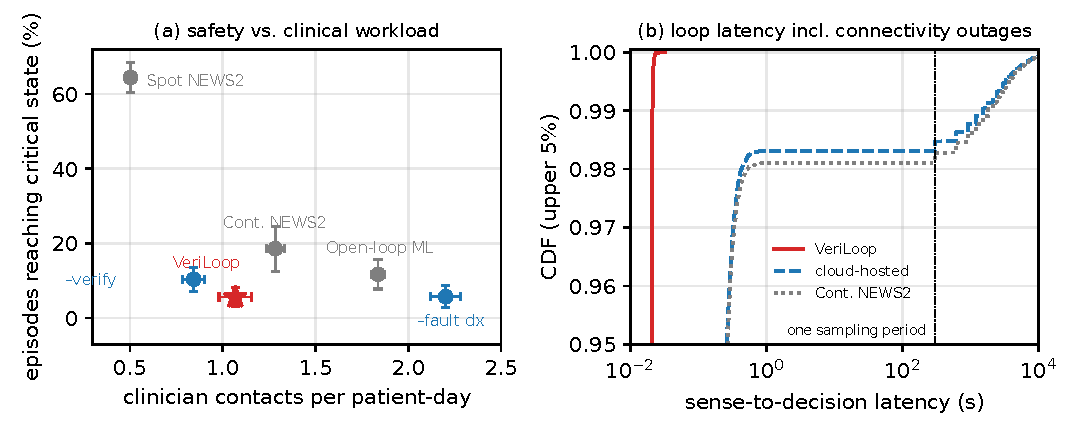
\includegraphics[width=0.82\textwidth]{figures/results.pdf}
\caption{(a) Share of episodes reaching a critical state versus clinician contacts per patient-day (95\% CIs over five
seeds). (b) Upper tail of the sense-to-decision latency distribution. Cloud-hosted designs wait for connectivity
outages to end; the edge loop does not.}
\label{fig:results}
\end{figure*}

\subsection*{Safety and Alarm Burden}

Periodic spot checks, the norm in many telemonitoring programmes, missed 28\% of episodes outright, and 64\% of
episodes became critical. Continuous NEWS2 alerted on every episode but did so late (median 2.9 hours before the
critical point) because NEWS2 crosses its amber threshold only once several vital signs are clearly abnormal, and 18.6\%
of episodes became critical. The personalised risk model in the open-loop ML design alerted earlier (4.6 hours) and
lowered the adverse-event rate to 11.7\%, at the cost of the highest false-alarm rate (1.49 per patient-day) and the
heaviest clinician workload.

VeriLoop let 5.7\% of episodes become critical: 23 of 409, against 74 for continuous NEWS2 (Fisher's exact test,
$p<10^{-7}$) and 47 for open-loop ML ($p=0.004$). At the same time it produced 0.59 false alarms per patient-day, 38\%
fewer than continuous NEWS2 and 60\% fewer than open-loop ML, which more than doubled alert precision to 33\%.
Fig.~\ref{fig:results}(a) shows that VeriLoop is the only design in the lower-left region: low adverse-event rate at a
clinical workload close to that of continuous NEWS2.

The price is paid in two places. Confirming a trigger with a re-measurement first costs about 18 minutes of lead time
relative to open-loop ML (4.3 versus 4.6 hours). And part of the burden moves from clinicians to patients: 1.4
re-measurement requests and 1.1 device checks per patient-day. Whether patients will accept that load is a
human-factors question the simulation cannot answer.

\begin{figure}[!t]
\centering
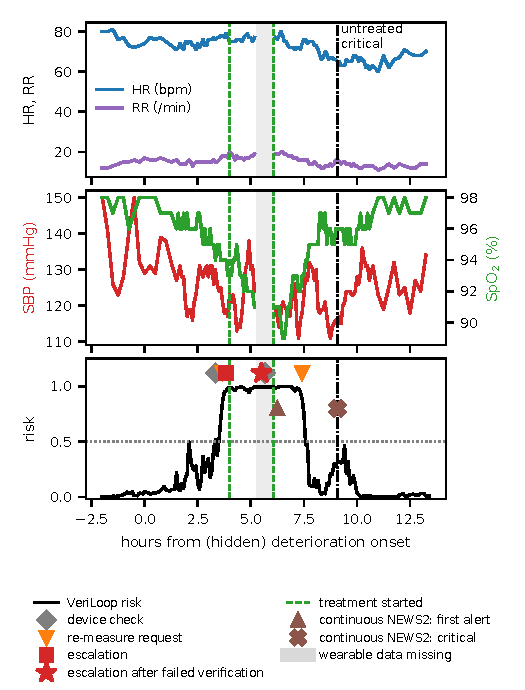
\includegraphics[width=\columnwidth]{figures/case_trace.pdf}
\caption{One simulated loop trace (respiratory deterioration). An early SpO$_2$ fall is first treated as a suspect
reading and checked, then confirmed by re-measurement and escalated. The first treatment fails; outcome verification
detects this 90 minutes later and escalates again, and the second treatment works. Under continuous NEWS2 the same
patient is first alerted 2.4 hours later and reaches the critical state.}
\label{fig:case}
\end{figure}

\subsection*{What Each Loop Stage Contributes}


\textbf{Outcome verification is where most of the safety gain comes from.} Without it, the adverse-event rate rose
from 5.7\% to 10.4\% (43 of 409 episodes, $p=0.014$), close to that of open-loop ML. Fig.~\ref{fig:case} shows the
mechanism. A failed first treatment is otherwise noticed only when the 4-hour alarm cooldown expires. With verification,
it is caught 90 minutes after treatment starts. Verification-triggered escalations were rare (0.07 per patient-day)
and 99\% of them occurred during a real episode. They do add workload, though. The full loop used 0.22 more clinician
contacts per patient-day than the variant without verification, and averaged 2.7 treatment contacts per episode
against 2.1. Part of this comes from verifying too early, before an effective treatment has fully taken hold, and a
verification window matched to each intervention would reduce it.

\textbf{Fault diagnosis and data confirmation do not change safety but halve the noise.} Removing them left the
adverse-event rate unchanged but nearly tripled false alarms (1.68 per patient-day) and doubled clinician contacts.
Fault-related false alarms fell five-fold, from 1.04 to 0.21 per patient-day. Because the edge asks patients to re-seat
or reconnect sensors, the time the cohort spent with corrupted data fell from 4.3 to 2.2 hours per patient-day. At
the sample-and-channel level, the edge pipeline flagged faults with 71\% precision and 69\% recall, against 40\% recall
for range checks alone. The imperfect precision matters: in Fig.~\ref{fig:case} a genuine SpO$_2$ fall was first
treated as suspect, and only the re-measurement prevented a delay.

\textbf{Bounded adaptation trims alarms safely.} Raising the personal threshold after confirmed false alarms reduced
false alarms by 19\% (0.73 to 0.59 per patient-day) without a detectable change in safety. Thresholds moved
modestly (mean final risk threshold 0.54) because the guardrails cap them.

\textbf{The edge buys resilience and bandwidth, not outcomes, in this setting.} Hosting the same loop in the cloud did
not change the adverse-event rate, because home outages (tens of minutes) are short compared with deteriorations that
develop over hours. It did, however, leave 1.7\% of samples waiting more than a minute, with a 99th-percentile latency
of about 16 minutes, compared with 21~ms at the edge (Fig.~\ref{fig:results}(b)). It also needed 30\% more uplink
traffic. For faster-moving conditions such as arrhythmia, falls or insulin delivery, that tail would matter clinically.

\textbf{Adaptive sampling halves sensing at no measurable safety cost.} Sampling every 15 minutes while stable kept the
wearable's sensing duty at 54\% of continuous operation. The difference in adverse-event rate against always-on sampling
($+1.2\pm4.5$ percentage points) was not significant. Overall, VeriLoop uploaded 11.6~KB per patient-day, against 28.1~KB
for continuous streaming.

\subsection*{Cost of Auditability}

The provenance ledger recorded about 294 entries per patient-day (152 bytes each, 44~KB per patient-day). Appending an
entry took 1.5~$\mu$s and verifying a full patient-week took 2.5~ms in unoptimised Python on a laptop-class CPU, which is
negligible next to the loop period. In 1,000 random tampering attempts on a patient-week log (modifying, deleting or
reordering entries, or truncating the tail), verification against the hourly cloud anchors detected all of them.
Truncation is detectable only back to the last anchor, so the anchor interval bounds how much of the log could be
silently dropped.


\section*{Lessons, Limitations and Open Challenges}


\textbf{Validation is a design stage, not a dashboard.} The largest single gain came from checking whether an action
worked. This is cheap to implement and fits naturally into the service-request lifecycle that FHIR \texttt{Task}
resources already describe~\cite{fhir}. Every RPM service should define, per action, what recovery is expected and
by when.

\textbf{Adaptation needs a declared envelope.} VeriLoop's personal thresholds can only move in one direction, by
fixed steps, within caps, and never touch red-flag rules. Expressing adaptation this way turns ``a learning system'' into
a reviewable list of permitted changes. That is what regulators now ask of adaptive medical software~\cite{fda2021},
and the provenance ledger provides the evidence that the envelope was respected.

\textbf{Loops redistribute work.} Confirmation and device checks lowered clinician workload by shifting effort to
patients. Service contracts should state that trade-off explicitly, and pilots should measure patient burden and
adherence, not just alarm counts.

\textbf{Limitations.} All results come from simulation. The physiology, faults and human behaviour are parameterised
models, and the clinician is assumed to recognise deterioration perfectly once it is apparent. The near-perfect
discrimination of the risk model reflects the simulator, not real data. The comparisons between designs are controlled
and paired, but absolute rates should not be read as clinical predictions. Security was evaluated only for log
integrity. Confidentiality, device authentication and key management, and attacks on an unanchored edge log within the
anchor interval (which hardware-backed signing would close), remain open.

\textbf{Open challenges.} Three questions deserve community attention. First, \emph{benchmarks}: closed-loop health
services cannot be evaluated on static datasets alone, and shared simulators calibrated against real RPM cohorts are
needed. Second, \emph{governance}: when a loop asks a patient to act and they do not, who is accountable, and how
should the loop escalate? Third, \emph{interoperable service contracts}: tiers, deadlines and verification rules
should be exchangeable between vendors and care providers as standard resources, not hard-coded in each platform.


\section*{Conclusion}


Device-centric remote monitoring stops at the alert. VeriLoop closes the loop by validating the data before acting,
verifying the outcome after acting, adapting only within declared bounds, and recording every step in a tamper-evident
ledger. In a controlled simulation with realistic sensor faults and connectivity outages, these mechanisms together
reduced the share of deteriorations reaching a critical state by more than two-thirds relative to continuous NEWS2
monitoring while lowering false alarms. Outcome verification was the most important single stage. The next step is to
calibrate the simulator against real RPM data and to test the loop in a supervised home-care pilot.


\section*{Code and Data Availability}
The simulator, VeriLoop implementation, experiment scripts and raw results are provided with this article
(repository link to be added on acceptance).

\bibliographystyle{IEEEtran}
\bibliography{refs}

\end{document}
